%D�finir le format du document: papier, taille de police, type de document, etc.
\documentclass[a4paper, 11pt]{article}

%%%%%%%%% Packages externes utilis�s %%%%%%%%%%%%%%%%%%%
\usepackage[french]{babel}
\usepackage[latin1]{inputenc}
\usepackage[T1]{fontenc}
\usepackage{verbatim}
\usepackage{graphicx}
\usepackage{epstopdf}
\usepackage{amsmath}
\usepackage{amssymb}
\usepackage{macro}
\usepackage{algorithm}
\usepackage{algorithmic}
%\usepackage{algorithm2e}


%La mise en page du rapport, NE PAS MODIFIER.
\usepackage{geometry}
 \geometry{
 a4paper,
 left=20mm,
 right=20mm,
 top=20mm,
 bottom=20mm,
 }

%%%%%%%%% Le corps du document entre begin et end %%%%%%%%%%%%%%%%%%%
\begin{document}

\section*{MAVLINK}
\label{sec:MAVLINK}

\noindent MAVLink (Micro Air Vehicle Link) is a communication protocol for small autonomous vehicles. It is mainly used in GCS communications <-> Unmanned Vehicle.

\subsection*{Protocol}
\label{sec:Protocol}

\paragraph{} The sent frames are divided into 8 main fields as shown in the following diagram:


\begin{figure}[H]
	\centering
		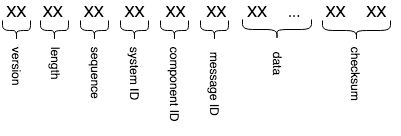
\includegraphics[scale=0.6]{./images/frame.png}
		\caption{The fields' names}
	\label{fig:frame}
\end{figure}

\paragraph{} For all this fields, we have a description and a range of values :

\begin{figure}[H]
	\centering
		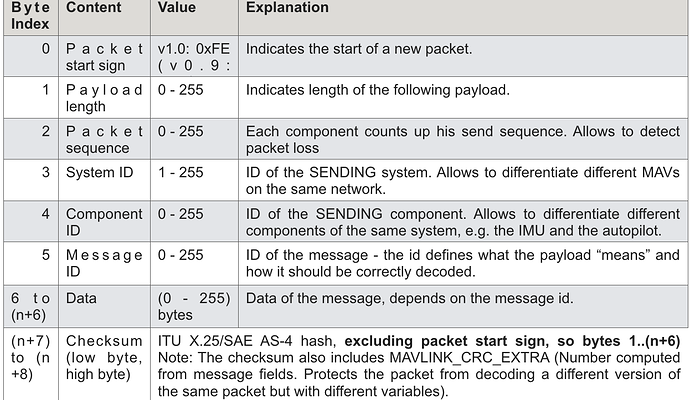
\includegraphics[scale=0.9]{./images/explanation.png}
		\caption{Explanation}
	\label{fig:explanation}
\end{figure}

\paragraph{} In our case some fields will remain unchanged, thus :
\begin{itemize}
\item Start sign stay at "fe" because we are working on version 1 of mavlink
\item System ID stay at "ff" because we simulate QGroundControl
\item Component ID stay at "00" too
\end{itemize}

\paragraph{} More the the message ID takes a value from those defined. (see sources)



\subsection*{Sources}
\label{sec:Sources}

\begin{itemize}
\item Explanation table : https://discuss.ardupilot.org/t/mavlink-step-by-step/9629
\item Message ID macro and values :  https://groups.google.com/forum/\#!topic/mavlink/1zgHUM67E-A
\end{itemize}




\end{document}
